\frame{
\frametitle{Result}%此页的标题

\begin{figure}
	\begin{center}
		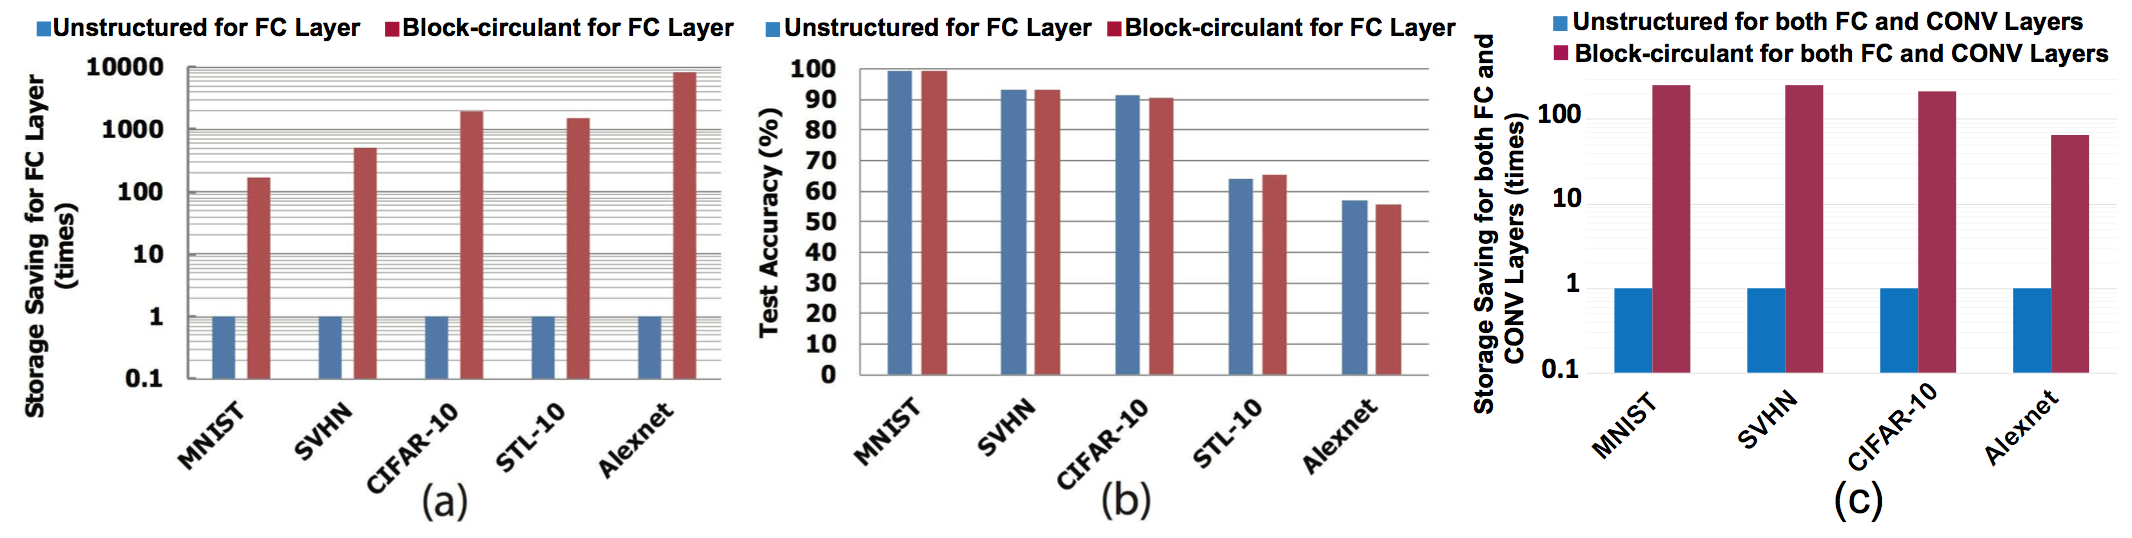
\includegraphics[width=1.01\linewidth]{Picture/result.png}
		\caption{(a) Storage saving and (b) test accuracy after using block-circulant FC layer for DCNN models on di erent datasets. (c) Storage saving after using both block-circulant FC layer and block-circulant CONV layer for DCNNs on MNIST, SVHN, CIFAR-10, and ImageNet datasets.}
		\label{Fig:3}
	\end{center}
	% \vspace{-0.1em}
\end{figure}

% \begin{eqnarray}
% 	% a_{5} &=& f\left( W_{51}\cdot X_{1}+W_{52}\cdot X_{2}+W_{53}\cdot X_{3}+W_{54}\cdot X_{4}\right)\\
% 	Y\left( x,y,p\right) =\sum ^{r}_{i=1}\sum ^{r}_{j=1}\sum ^{c}_{c=1}F\left( i,j,c,p\right) X\left( x+i-1,y+j-1,c\right)
% \end{eqnarray}

}